% Options for packages loaded elsewhere
\PassOptionsToPackage{unicode}{hyperref}
\PassOptionsToPackage{hyphens}{url}
%
\documentclass[
]{book}
\usepackage{amsmath,amssymb}
\usepackage{lmodern}
\usepackage{iftex}
\ifPDFTeX
  \usepackage[T1]{fontenc}
  \usepackage[utf8]{inputenc}
  \usepackage{textcomp} % provide euro and other symbols
\else % if luatex or xetex
  \usepackage{unicode-math}
  \defaultfontfeatures{Scale=MatchLowercase}
  \defaultfontfeatures[\rmfamily]{Ligatures=TeX,Scale=1}
\fi
% Use upquote if available, for straight quotes in verbatim environments
\IfFileExists{upquote.sty}{\usepackage{upquote}}{}
\IfFileExists{microtype.sty}{% use microtype if available
  \usepackage[]{microtype}
  \UseMicrotypeSet[protrusion]{basicmath} % disable protrusion for tt fonts
}{}
\makeatletter
\@ifundefined{KOMAClassName}{% if non-KOMA class
  \IfFileExists{parskip.sty}{%
    \usepackage{parskip}
  }{% else
    \setlength{\parindent}{0pt}
    \setlength{\parskip}{6pt plus 2pt minus 1pt}}
}{% if KOMA class
  \KOMAoptions{parskip=half}}
\makeatother
\usepackage{xcolor}
\IfFileExists{xurl.sty}{\usepackage{xurl}}{} % add URL line breaks if available
\IfFileExists{bookmark.sty}{\usepackage{bookmark}}{\usepackage{hyperref}}
\hypersetup{
  pdftitle={Introducción a la fonética del español},
  pdfauthor={Joseph V. Casillas},
  hidelinks,
  pdfcreator={LaTeX via pandoc}}
\urlstyle{same} % disable monospaced font for URLs
\usepackage{longtable,booktabs,array}
\usepackage{calc} % for calculating minipage widths
% Correct order of tables after \paragraph or \subparagraph
\usepackage{etoolbox}
\makeatletter
\patchcmd\longtable{\par}{\if@noskipsec\mbox{}\fi\par}{}{}
\makeatother
% Allow footnotes in longtable head/foot
\IfFileExists{footnotehyper.sty}{\usepackage{footnotehyper}}{\usepackage{footnote}}
\makesavenoteenv{longtable}
\usepackage{graphicx}
\makeatletter
\def\maxwidth{\ifdim\Gin@nat@width>\linewidth\linewidth\else\Gin@nat@width\fi}
\def\maxheight{\ifdim\Gin@nat@height>\textheight\textheight\else\Gin@nat@height\fi}
\makeatother
% Scale images if necessary, so that they will not overflow the page
% margins by default, and it is still possible to overwrite the defaults
% using explicit options in \includegraphics[width, height, ...]{}
\setkeys{Gin}{width=\maxwidth,height=\maxheight,keepaspectratio}
% Set default figure placement to htbp
\makeatletter
\def\fps@figure{htbp}
\makeatother
\setlength{\emergencystretch}{3em} % prevent overfull lines
\providecommand{\tightlist}{%
  \setlength{\itemsep}{0pt}\setlength{\parskip}{0pt}}
\setcounter{secnumdepth}{5}
\usepackage[spanish]{babel}


\usepackage{booktabs}
\usepackage{longtable}
\usepackage[bf,singlelinecheck=off]{caption}


\usepackage{framed,color}
\definecolor{shadecolor}{RGB}{240,240,240}

\renewcommand{\textfraction}{0.05}
\renewcommand{\topfraction}{0.8}
\renewcommand{\bottomfraction}{0.8}
\renewcommand{\floatpagefraction}{0.75}

\renewenvironment{quote}{\begin{VF}}{\end{VF}}
\let\oldhref\href
\renewcommand{\href}[2]{#2\footnote{\url{#1}}}

\ifxetex
  \usepackage{letltxmacro}
  \setlength{\XeTeXLinkMargin}{1pt}
  \LetLtxMacro\SavedIncludeGraphics\includegraphics
  \def\includegraphics#1#{% #1 catches optional stuff (star/opt. arg.)
    \IncludeGraphicsAux{#1}%
  }%
  \newcommand*{\IncludeGraphicsAux}[2]{%
    \XeTeXLinkBox{%
      \SavedIncludeGraphics#1{#2}%
    }%
  }%
\fi

\makeatletter
\newenvironment{kframe}{%
\medskip{}
\setlength{\fboxsep}{.8em}
 \def\at@end@of@kframe{}%
 \ifinner\ifhmode%
  \def\at@end@of@kframe{\end{minipage}}%
  \begin{minipage}{\columnwidth}%
 \fi\fi%
 \def\FrameCommand##1{\hskip\@totalleftmargin \hskip-\fboxsep
 \colorbox{shadecolor}{##1}\hskip-\fboxsep
     % There is no \\@totalrightmargin, so:
     \hskip-\linewidth \hskip-\@totalleftmargin \hskip\columnwidth}%
 \MakeFramed {\advance\hsize-\width
   \@totalleftmargin\z@ \linewidth\hsize
   \@setminipage}}%
 {\par\unskip\endMakeFramed%
 \at@end@of@kframe}
\makeatother

\makeatletter
\@ifundefined{Shaded}{
}{\renewenvironment{Shaded}{\begin{kframe}}{\end{kframe}}}
\makeatother

\newenvironment{rmdblock}[1]
  {
  \begin{itemize}
  \renewcommand{\labelitemi}{
    \raisebox{-.7\height}[0pt][0pt]{
      {\setkeys{Gin}{width=3em,keepaspectratio}\includegraphics{assets/images/#1}}
    }
  }
  \setlength{\fboxsep}{1em}
  \begin{kframe}
  \item
  }
  {
  \end{kframe}
  \end{itemize}
  }
\newenvironment{rmdojo}
  {\begin{rmdblock}{ojo}}
  {\end{rmdblock}}
\newenvironment{rmdbomb}
  {\begin{rmdblock}{bomb}}
  {\end{rmdblock}}
\newenvironment{rmdexercise}
  {\begin{rmdblock}{exercise}}
  {\end{rmdblock}}
\newenvironment{rmdteach}
  {\begin{rmdblock}{teach}}
  {\end{rmdblock}}
\newenvironment{rmdwarning}
  {\begin{rmdblock}{warning}}
  {\end{rmdblock}}

\usepackage{makeidx}
\makeindex

\urlstyle{tt}

\usepackage{amsthm}
\makeatletter
\def\thm@space@setup{%
  \thm@preskip=8pt plus 2pt minus 4pt
  \thm@postskip=\thm@preskip
}
\makeatother

\frontmatter
\ifLuaTeX
  \usepackage{selnolig}  % disable illegal ligatures
\fi
\usepackage[]{natbib}
\bibliographystyle{apalike}

\title{Introducción a la fonética del español}
\author{Joseph V. Casillas}
\date{2022-01-12}

\begin{document}
\maketitle

\thispagestyle{empty}

\begin{center}

\includegraphics{assets/images/oat_logo.png}
\end{center}

\setlength{\abovedisplayskip}{-5pt}
\setlength{\abovedisplayshortskip}{-5pt}

{
\setcounter{tocdepth}{1}
\tableofcontents
}
\hypertarget{acerca-de-este-libro}{%
\chapter*{Acerca de este libro}\label{acerca-de-este-libro}}
\addcontentsline{toc}{chapter}{Acerca de este libro}

This course has received an `Open and Affordable Textbooks Program' award from
the Rutgers University Libraries.
The OAT Program supports textbook affordability at Rutgers by encouraging
courses to adopt educational materials that are freely available, available at
a low cost (compared to similar courses), or part of the Rutgers University
Libraries' electronic collections, and thereby free of charge to Rutgers
University students.
As a student in this course, you will be asked to provide feedback on this
initiative at the end of the semester.

\begin{center}
\includegraphics[width=0.33\linewidth]{/Users/casillas/academia/teaching/rutgers/spanphon/oat/assets/images/oat_logo} \end{center}

\hypertarget{cuxf3mo-leer-este-libro}{%
\section*{Cómo leer este libro}\label{cuxf3mo-leer-este-libro}}
\addcontentsline{toc}{section}{Cómo leer este libro}

Este libro está pensado para tres tipos de personas: el estudiante de español
como L2, el maestro de español como L2 y el aficionado que se interesa en
conocer la fonética y fonología del español.

\hypertarget{algunas-convenciones}{%
\section*{Algunas convenciones}\label{algunas-convenciones}}
\addcontentsline{toc}{section}{Algunas convenciones}

A lo largo del texto aparecerán las siguientes imágenes que sirven para indicar
al lector que algo acerca del texto que sigue a continuación.
A saber\ldots{}

\begin{figure}

{\centering 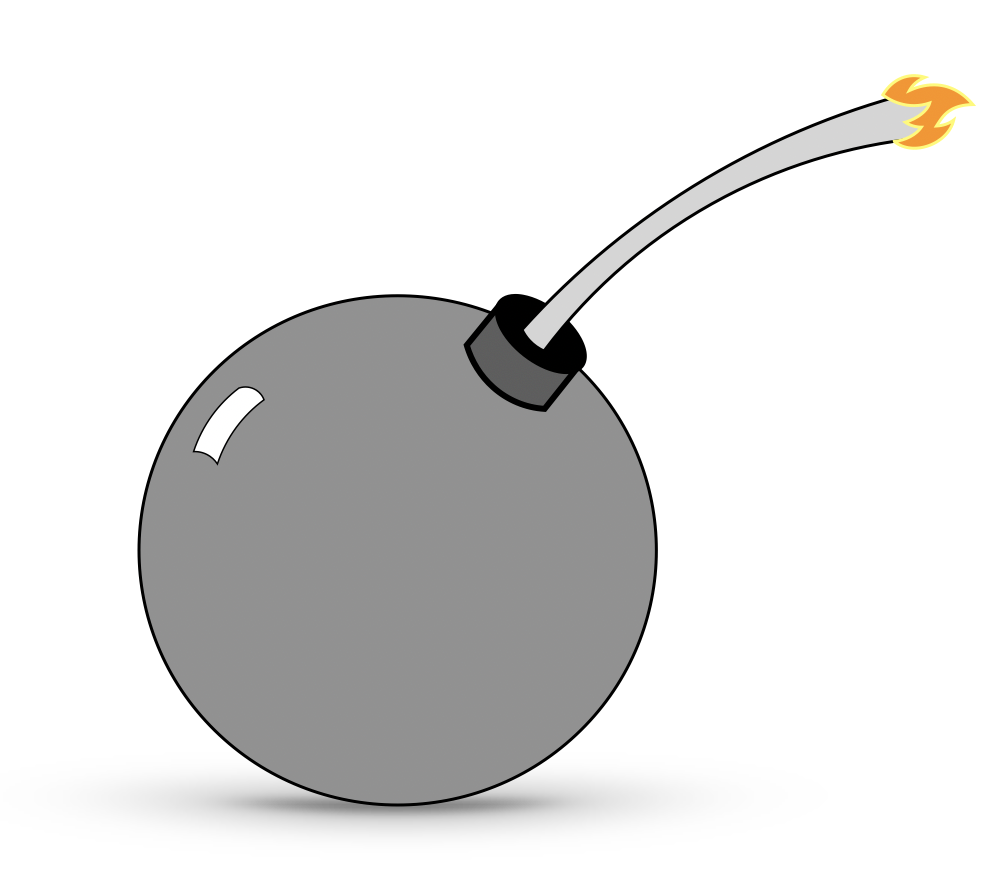
\includegraphics[width=0.2\linewidth]{/Users/casillas/academia/teaching/rutgers/spanphon/oat/assets/images/bomb} 
\includegraphics[width=0.2\linewidth]{/Users/casillas/academia/teaching/rutgers/spanphon/oat/assets/images/ojo} 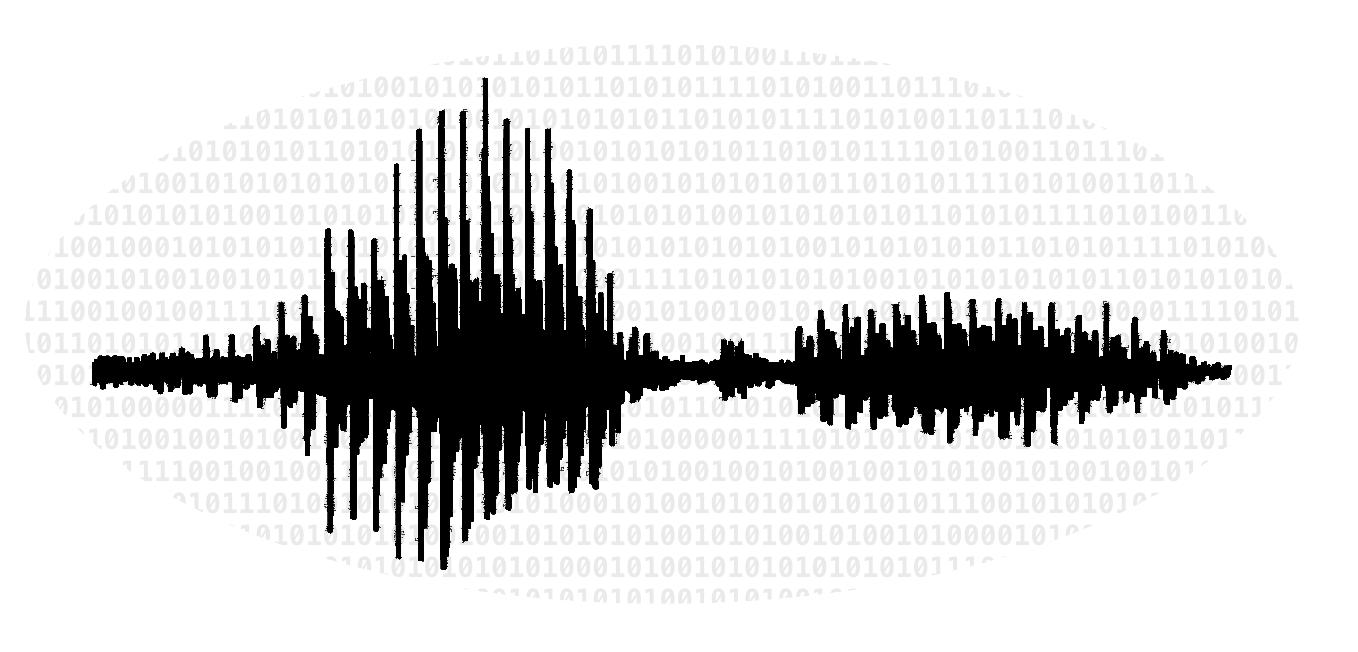
\includegraphics[width=0.2\linewidth]{/Users/casillas/academia/teaching/rutgers/spanphon/oat/assets/images/exercise} 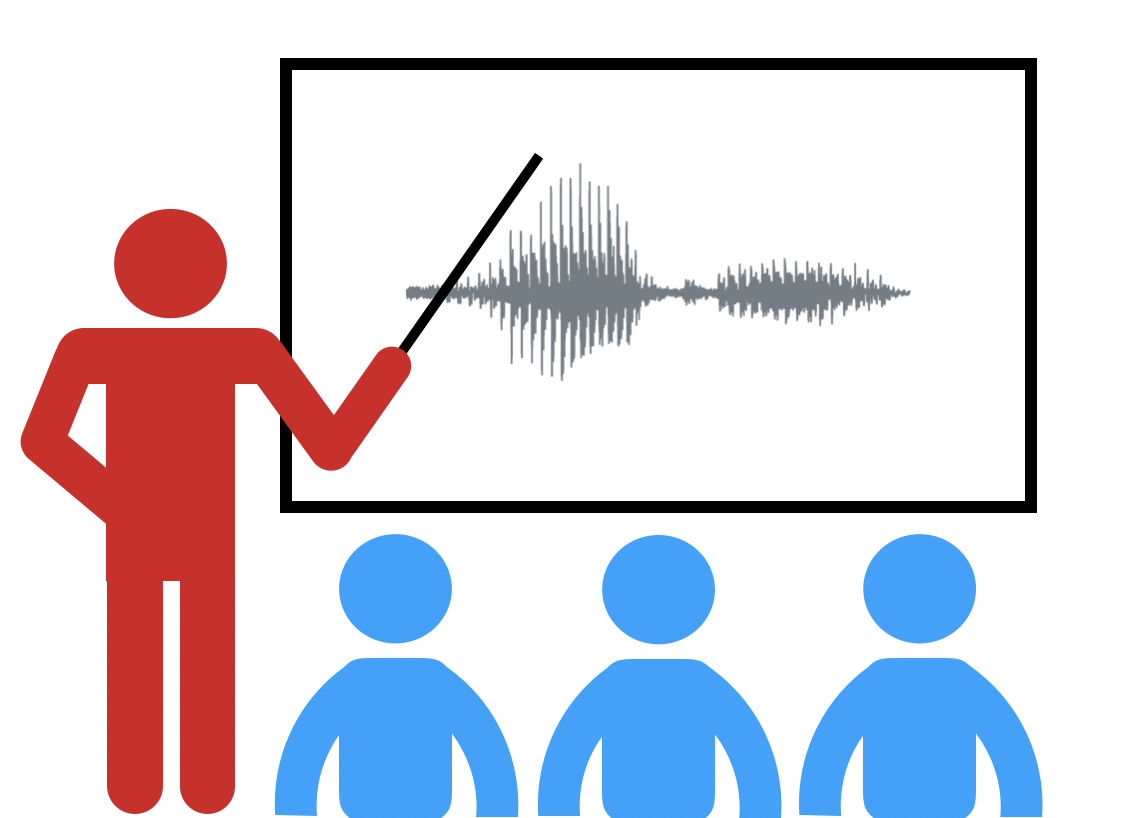
\includegraphics[width=0.2\linewidth]{/Users/casillas/academia/teaching/rutgers/spanphon/oat/assets/images/teach} 

}

\caption{test caption}\label{fig:bloques}
\end{figure}

\begin{rmdojo}
Un bloque de texto así, que contiene un punto de exclamación al lado,
implica que aquí va información importante que debe leerse. Como regla
general es mejor no prescindir de estas secciones porque cuentan con
información que vas a querer saber.
\end{rmdojo}

\begin{rmdbomb}
Al ver un bloque de texto que contiene una bomba al lado, el lector ha
de suponer que el contenido de esta sección es difícil y puede resultar
confuso para muchos estudiantes. El tipo de información que suele
aparecer en estos bloques sirve para generar fantásticas preguntas para
los exámenes.
\end{rmdbomb}

\begin{rmdexercise}
Al ver un bloque de texto que contiene una bomba al lado, el lector ha
de suponer que el contenido de esta sección es difícil y puede resultar
confuso para muchos estudiantes. El tipo de información que suele
aparecer en estos bloques sirve para generar fantásticas preguntas para
los exámenes.
\end{rmdexercise}

\begin{rmdteach}
Al ver un bloque de texto que contiene una bomba al lado, el lector ha
de suponer que el contenido de esta sección es difícil y puede resultar
confuso para muchos estudiantes. El tipo de información que suele
aparecer en estos bloques sirve para generar fantásticas preguntas para
los exámenes.
\end{rmdteach}

\citet{xie2015}

\hypertarget{intro}{%
\chapter{¿Qué es la lingüística?}\label{intro}}

La lingüística es\ldots{}

\hypertarget{ramas}{%
\section{Ramas}\label{ramas}}

Lorem ipsum dolor sit amet, consectetur adipisicing elit, sed do eiusmod
tempor incididunt ut labore et dolore magna aliqua. Ut enim ad minim veniam,
quis nostrud exercitation ullamco laboris nisi ut aliquip ex ea commodo
consequat. Duis aute irure dolor in reprehenderit in voluptate velit esse
cillum dolore eu fugiat nulla pariatur. Excepteur sint occaecat cupidatat non
proident, sunt in culpa qui officia deserunt mollit anim id est laborum.

\hypertarget{el-estudio-del-lenguaje}{%
\section{El estudio del lenguaje}\label{el-estudio-del-lenguaje}}

Lorem ipsum dolor sit amet, consectetur adipisicing elit, sed do eiusmod
tempor incididunt ut labore et dolore magna aliqua. Ut enim ad minim veniam,
quis nostrud exercitation ullamco laboris nisi ut aliquip ex ea commodo
consequat. Duis aute irure dolor in reprehenderit in voluptate velit esse
cillum dolore eu fugiat nulla pariatur. Excepteur sint occaecat cupidatat non
proident, sunt in culpa qui officia deserunt mollit anim id est laborum.

\hypertarget{silaba}{%
\chapter{La sílaba, los diptongos y los hiatos}\label{silaba}}

\hypertarget{la-suxedlaba}{%
\section{La sílaba}\label{la-suxedlaba}}

Lorem ipsum dolor sit amet, consectetur adipisicing elit, sed do eiusmod
tempor incididunt ut labore et dolore magna aliqua. Ut enim ad minim veniam,
quis nostrud exercitation ullamco laboris nisi ut aliquip ex ea commodo
consequat. Duis aute irure dolor in reprehenderit in voluptate velit esse
cillum dolore eu fugiat nulla pariatur. Excepteur sint occaecat cupidatat non
proident, sunt in culpa qui officia deserunt mollit anim id est laborum.

\hypertarget{los-diptongos}{%
\section{Los diptongos}\label{los-diptongos}}

Lorem ipsum dolor sit amet, consectetur adipisicing elit, sed do eiusmod
tempor incididunt ut labore et dolore magna aliqua. Ut enim ad minim veniam,
quis nostrud exercitation ullamco laboris nisi ut aliquip ex ea commodo
consequat. Duis aute irure dolor in reprehenderit in voluptate velit esse
cillum dolore eu fugiat nulla pariatur. Excepteur sint occaecat cupidatat non
proident, sunt in culpa qui officia deserunt mollit anim id est laborum.

\hypertarget{los-hiatos}{%
\section{Los hiatos}\label{los-hiatos}}

Lorem ipsum dolor sit amet, consectetur adipisicing elit, sed do eiusmod
tempor incididunt ut labore et dolore magna aliqua. Ut enim ad minim veniam,
quis nostrud exercitation ullamco laboris nisi ut aliquip ex ea commodo
consequat. Duis aute irure dolor in reprehenderit in voluptate velit esse
cillum dolore eu fugiat nulla pariatur. Excepteur sint occaecat cupidatat non
proident, sunt in culpa qui officia deserunt mollit anim id est laborum.

\hypertarget{acustica-basica}{%
\chapter{Algunas nociones de la fonética acústica, el hardware y el software}\label{acustica-basica}}

\hypertarget{acuxfastica}{%
\section{¿Acústica?}\label{acuxfastica}}

Lorem ipsum dolor sit amet, consectetur adipisicing elit, sed do eiusmod
tempor incididunt ut labore et dolore magna aliqua. Ut enim ad minim veniam,
quis nostrud exercitation ullamco laboris nisi ut aliquip ex ea commodo
consequat. Duis aute irure dolor in reprehenderit in voluptate velit esse
cillum dolore eu fugiat nulla pariatur. Excepteur sint occaecat cupidatat non
proident, sunt in culpa qui officia deserunt mollit anim id est laborum.

\hypertarget{hardware}{%
\section{Hardware}\label{hardware}}

Lorem ipsum dolor sit amet, consectetur adipisicing elit, sed do eiusmod
tempor incididunt ut labore et dolore magna aliqua. Ut enim ad minim veniam,
quis nostrud exercitation ullamco laboris nisi ut aliquip ex ea commodo
consequat. Duis aute irure dolor in reprehenderit in voluptate velit esse
cillum dolore eu fugiat nulla pariatur. Excepteur sint occaecat cupidatat non
proident, sunt in culpa qui officia deserunt mollit anim id est laborum.

\hypertarget{software}{%
\section{Software}\label{software}}

Lorem ipsum dolor sit amet, consectetur adipisicing elit, sed do eiusmod
tempor incididunt ut labore et dolore magna aliqua. Ut enim ad minim veniam,
quis nostrud exercitation ullamco laboris nisi ut aliquip ex ea commodo
consequat. Duis aute irure dolor in reprehenderit in voluptate velit esse
cillum dolore eu fugiat nulla pariatur. Excepteur sint occaecat cupidatat non
proident, sunt in culpa qui officia deserunt mollit anim id est laborum.

\hypertarget{descripcion-articulatoria}{%
\chapter{La fonética articulatoria}\label{descripcion-articulatoria}}

\hypertarget{la-descripciuxf3n-articulatoria}{%
\section{La descripción articulatoria}\label{la-descripciuxf3n-articulatoria}}

Lorem ipsum dolor sit amet, consectetur adipisicing elit, sed do eiusmod
tempor incididunt ut labore et dolore magna aliqua. Ut enim ad minim veniam,
quis nostrud exercitation ullamco laboris nisi ut aliquip ex ea commodo
consequat. Duis aute irure dolor in reprehenderit in voluptate velit esse
cillum dolore eu fugiat nulla pariatur. Excepteur sint occaecat cupidatat non
proident, sunt in culpa qui officia deserunt mollit anim id est laborum.

\hypertarget{las-vocales}{%
\section{Las vocales}\label{las-vocales}}

Lorem ipsum dolor sit amet, consectetur adipisicing elit, sed do eiusmod
tempor incididunt ut labore et dolore magna aliqua. Ut enim ad minim veniam,
quis nostrud exercitation ullamco laboris nisi ut aliquip ex ea commodo
consequat. Duis aute irure dolor in reprehenderit in voluptate velit esse
cillum dolore eu fugiat nulla pariatur. Excepteur sint occaecat cupidatat non
proident, sunt in culpa qui officia deserunt mollit anim id est laborum.

\hypertarget{las-consonantes}{%
\section{Las consonantes}\label{las-consonantes}}

Lorem ipsum dolor sit amet, consectetur adipisicing elit, sed do eiusmod
tempor incididunt ut labore et dolore magna aliqua. Ut enim ad minim veniam,
quis nostrud exercitation ullamco laboris nisi ut aliquip ex ea commodo
consequat. Duis aute irure dolor in reprehenderit in voluptate velit esse
cillum dolore eu fugiat nulla pariatur. Excepteur sint occaecat cupidatat non
proident, sunt in culpa qui officia deserunt mollit anim id est laborum.

\hypertarget{obstruyentes}{%
\chapter{Las obstruyentes}\label{obstruyentes}}

\hypertarget{las-oclusivas}{%
\section{Las oclusivas}\label{las-oclusivas}}

Lorem ipsum dolor sit amet, consectetur adipisicing elit, sed do eiusmod
tempor incididunt ut labore et dolore magna aliqua. Ut enim ad minim veniam,
quis nostrud exercitation ullamco laboris nisi ut aliquip ex ea commodo
consequat. Duis aute irure dolor in reprehenderit in voluptate velit esse
cillum dolore eu fugiat nulla pariatur. Excepteur sint occaecat cupidatat non
proident, sunt in culpa qui officia deserunt mollit anim id est laborum.

\hypertarget{fricativas-estridentes}{%
\section{Fricativas estridentes}\label{fricativas-estridentes}}

Lorem ipsum dolor sit amet, consectetur adipisicing elit, sed do eiusmod
tempor incididunt ut labore et dolore magna aliqua. Ut enim ad minim veniam,
quis nostrud exercitation ullamco laboris nisi ut aliquip ex ea commodo
consequat. Duis aute irure dolor in reprehenderit in voluptate velit esse
cillum dolore eu fugiat nulla pariatur. Excepteur sint occaecat cupidatat non
proident, sunt in culpa qui officia deserunt mollit anim id est laborum.

\hypertarget{nasales-laterales}{%
\chapter{Las consonantes nasales y laterales}\label{nasales-laterales}}

\hypertarget{las-nasales}{%
\section{Las nasales}\label{las-nasales}}

Lorem ipsum dolor sit amet, consectetur adipisicing elit, sed do eiusmod
tempor incididunt ut labore et dolore magna aliqua. Ut enim ad minim veniam,
quis nostrud exercitation ullamco laboris nisi ut aliquip ex ea commodo
consequat. Duis aute irure dolor in reprehenderit in voluptate velit esse
cillum dolore eu fugiat nulla pariatur. Excepteur sint occaecat cupidatat non
proident, sunt in culpa qui officia deserunt mollit anim id est laborum.

\hypertarget{las-laterales}{%
\section{Las laterales}\label{las-laterales}}

Lorem ipsum dolor sit amet, consectetur adipisicing elit, sed do eiusmod
tempor incididunt ut labore et dolore magna aliqua. Ut enim ad minim veniam,
quis nostrud exercitation ullamco laboris nisi ut aliquip ex ea commodo
consequat. Duis aute irure dolor in reprehenderit in voluptate velit esse
cillum dolore eu fugiat nulla pariatur. Excepteur sint occaecat cupidatat non
proident, sunt in culpa qui officia deserunt mollit anim id est laborum.

\hypertarget{vibrantes}{%
\chapter{Las vibrantes}\label{vibrantes}}

rrrrr

\hypertarget{variacion-dialectal}{%
\chapter{La variación dialectal}\label{variacion-dialectal}}

\hypertarget{tres-zonas-dialectales}{%
\section{Tres zonas dialectales}\label{tres-zonas-dialectales}}

Lorem ipsum dolor sit amet, consectetur adipisicing elit, sed do eiusmod
tempor incididunt ut labore et dolore magna aliqua. Ut enim ad minim veniam,
quis nostrud exercitation ullamco laboris nisi ut aliquip ex ea commodo
consequat. Duis aute irure dolor in reprehenderit in voluptate velit esse
cillum dolore eu fugiat nulla pariatur. Excepteur sint occaecat cupidatat non
proident, sunt in culpa qui officia deserunt mollit anim id est laborum.

\hypertarget{tres-zonas-dialectales-1}{%
\section{¿Tres zonas dialectales?}\label{tres-zonas-dialectales-1}}

Lorem ipsum dolor sit amet, consectetur adipisicing elit, sed do eiusmod
tempor incididunt ut labore et dolore magna aliqua. Ut enim ad minim veniam,
quis nostrud exercitation ullamco laboris nisi ut aliquip ex ea commodo
consequat. Duis aute irure dolor in reprehenderit in voluptate velit esse
cillum dolore eu fugiat nulla pariatur. Excepteur sint occaecat cupidatat non
proident, sunt in culpa qui officia deserunt mollit anim id est laborum.

\hypertarget{el-espauxf1ol-andaluz}{%
\section{El español andaluz}\label{el-espauxf1ol-andaluz}}

Lorem ipsum dolor sit amet, consectetur adipisicing elit, sed do eiusmod
tempor incididunt ut labore et dolore magna aliqua. Ut enim ad minim veniam,
quis nostrud exercitation ullamco laboris nisi ut aliquip ex ea commodo
consequat. Duis aute irure dolor in reprehenderit in voluptate velit esse
cillum dolore eu fugiat nulla pariatur. Excepteur sint occaecat cupidatat non
proident, sunt in culpa qui officia deserunt mollit anim id est laborum.xw

  \bibliography{book.bib,packages.bib}

\printindex

\end{document}
